\section{Airplane Landing Problem}
 Let $x_1, x_2,...,x_n $ be the exact landing time of each airplane respectively, the problem can be written as 
 \[	\begin{split} 
	 \max  \quad &\min(x_2 - x_1, x_3 - x_2, ..., x_n - x_{n-1}) \\
	 \text{s.t.} \quad & s_1 \leq x_1 \leq t_1 \\
	 & s_2 \leq x_2 \leq t_2  \\
	 &\cdots \\
	 & s_n \leq x_n \leq t_n
	\end{split}  
 \]
 for instance, we have $n = 4, [10,20],[40,60],[75,80],[100,120]$ ( here the minute is the metric of time),
 using tool cvxpy we can obtain the optimal solution $35$ with optimal variables $x_1 = 10, 45,80,116$.
 \begin{figure}[H]
 	\centering
 	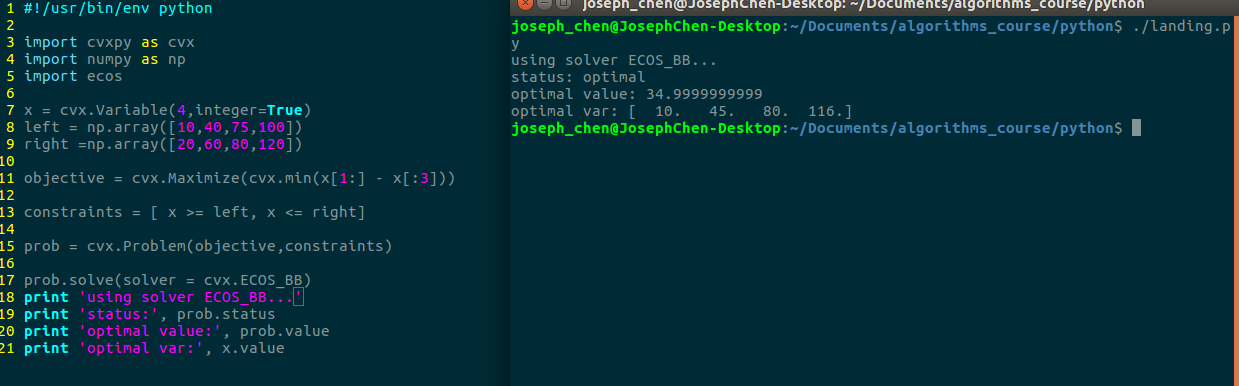
\includegraphics[width=.8\textwidth]{work4/landing}
 \end{figure}
